\documentclass[journal,10pt,twocolumn]{IEEEtran}
\IEEEoverridecommandlockouts

\usepackage{cite}
\usepackage{amsmath,amssymb,amsfonts}
\usepackage{algorithmic}
\usepackage{graphicx}
\usepackage{textcomp}
\usepackage{xcolor}
\usepackage{tikz}
\usetikzlibrary{arrows.meta, positioning, shapes.geometric, shapes.misc, calc, shadows}
\usepackage{booktabs}
\usepackage{tabularx}
\usepackage{url}
\usepackage{multirow}
\usepackage{microtype}
\usepackage{balance}

\begin{document}

\title{Agentic Graph RAG for Explainable Multimodal Clinical Decision Support with Verifiable Evidence and Client-Side Radiographic Saliency}

\author{Vikram~Kadam,
        Keshav~Mittal,
        Sandesh~Phad,
        Tejas~Shidam,
        and~Madhuri~Pagale\\
        \small\textit{Emails: \{vikramkadam23, keshavmittal23, sandeshphad23, tejasshidam23, madhuripagale\}@gmail.com}%
\thanks{V. Kadam, K. Mittal, S. Phad, and T. Shidam are undergraduate researchers in the Department of Computer Science \& Engineering (Artificial Intelligence \& Machine Learning), Pimpri Chinchwad College of Engineering (PCCOE), Pune 411044, India (e-mail: \{vikramkadam23, keshavmittal23, sandeshphad23, tejasshidam23\}@gmail.com; \{vikram.kadam23, keshav.mittal23, sandesh.phad23, tejas.shidam23\}@pccoepune.org).}%
\thanks{M. Pagale is an Assistant Professor in the Department of Computer Science \& Engineering (AI \& ML), Pimpri Chinchwad College of Engineering, Pune 411044, India (e-mail: madhuripagale@gmail.com, madhuri.pagale@pccoepune.org).}%
}

\markboth{Manuscript Submitted for Academic and Clinical Research Evaluation,~August~2026}%
{Kadam \MakeLowercase{\textit{et al.}}: Agentic Graph RAG for Explainable Multimodal Clinical Decision Support}

\maketitle

\begin{abstract}
While Large Language Models (LLMs) encode extensive biomedical knowledge, clinical deployment remains constrained by ungrounded hallucinations, absent literature provenance, opaque reasoning chains, uncalibrated confidence heuristics, and patient privacy risks during cloud-based multimodal inference. This paper presents \textbf{MEDGUIDE AI}, an explainable, multi-agent Clinical Decision Support System (CDSS) that unifies Retrieval-Augmented Generation (RAG) with structured clinical knowledge graphs, deterministic pharmacovigilance, and privacy-preserving client-side radiographic saliency. The proposed architecture coordinates 12 specialized workflow agents across diagnostic planning, multi-source biomedical literature retrieval (PubMed, Europe PMC, WHO, ClinicalTrials.gov), knowledge graph ontology traversal ($G=(V,E)$), deterministic pharmacology and allergy verification (openFDA, RxNorm), post-hoc safety auditing, and continuous benchmark evaluation. Diagnostic hypotheses are systematically grounded in retrieved medical sources classified under the Oxford Centre for Evidence-Based Medicine (CEBM) 5-tier schema. In addition, an in-browser DenseNet-121 neural model executing via WebAssembly generates occlusion sensitivity heatmaps on raw chest radiographs without transmitting image pixels to external servers for saliency localization. The framework evaluates a multi-signal composite confidence metric categorized into ordinal bands (High, Medium, Low, Insufficient Evidence). We established an evaluation protocol across 50 multi-system clinical vignettes. Experimental results indicate that Agentic Graph RAG achieves a 90.0\% evidence grounding rate, 92.0\% safety compliance, and 95.0\% system-defined explainability score, outperforming zero-shot LLMs (20.0\%, 35.0\%, 15.0\%) and standard vector RAG (65.0\%, 60.0\%, 55.0\%). The system maintains non-autonomous operational boundaries, incorporates a formal Model Facts specification, and aligns with principles outlined in the World Health Organization (WHO) 2024 guidance on Large Multi-Modal Models in healthcare.
\end{abstract}

\begin{IEEEkeywords}
Clinical Decision Support Systems, Explainable AI, Retrieval-Augmented Generation, Medical Knowledge Graphs, Multi-Agent Systems, Radiographic Saliency, Edge AI, Biomedical Informatics.
\end{IEEEkeywords}

\IEEEpeerreviewmaketitle

\section{Introduction}

\subsection{Clinical Decision Support Background}
\IEEEPARstart{C}{linical} Decision Support Systems (CDSS) represent an established area of biomedical informatics research \cite{shortliffe1975mycin, bates2003ten}. In modern healthcare settings, physicians encounter high patient volumes, compressed consultation windows, and rapid literature expansion, with over two million scientific articles indexed annually in MEDLINE \cite{topol2019high, bates2003ten}. Diagnostic discrepancies and therapeutic errors continue to affect inpatient admissions, with studies reporting diagnostic error rates between 10\% and 15\% in complex acute presentations \cite{bates2003ten, rajkomar2018scalable}. These errors often arise from cognitive heuristics, premature diagnostic closure, atypical symptom patterns, or unflagged drug-drug and drug-allergy interactions.

Early rule-based CDSS such as MYCIN \cite{shortliffe1975mycin} and DXplain established the feasibility of encoding expert heuristics for infectious disease management and differential diagnosis. Subsequent systems embedded statistical rule triggers within Electronic Health Record (EHR) workflows \cite{rajkomar2018scalable, sendak2020real}. However, static rule-based systems exhibited limited adaptability across diverse clinical narratives and suffered from high manual maintenance overhead. Furthermore, non-selective alerting thresholds frequently induced clinical alert fatigue, resulting in override rates exceeding 90\% in hospital deployments \cite{bates2003ten, sendak2020real}.

\subsection{Limitations of Generative LLMs in Medical Practice}
Recent progress in biomedical Large Language Models (LLMs), including Med-PaLM 2 \cite{singhal2023large}, Med-Gemini \cite{saab2024capabilities}, and AMIE \cite{tu2024towards}, has demonstrated high factual performance on medical licensing benchmarks \cite{holmes2023evaluating}. In a double-blind crossover trial published in \textit{Nature}, Tu et al. \cite{tu2024towards} observed that the conversational diagnostic model AMIE achieved diagnostic accuracy and consultation quality comparable to primary-care physicians across simulated clinical consultations.

Despite these capabilities, ungrounded generative models exhibit specific technical limitations when applied to direct clinical workflows:
\begin{enumerate}
    \item \textbf{Stochastic Hallucinations:} Parametric language models sample text probabilistically, occasionally generating fictitious clinical findings, fabricated trial identifiers (NCT numbers), or invalid PubMed IDs with fluent syntax \cite{singhal2023large, wu2025medical}.
    \item \textbf{Lack of Verifiable Grounding:} Monolithic LLM generations lack direct, auditable links to authoritative clinical practice guidelines (e.g., NICE, WHO, ESC, ACC/AHA) or peer-reviewed primary literature, preventing clinicians from inspecting the evidentiary basis of generated assertions \cite{edge2024from, liao2024dapr}.
    \item \textbf{Uncalibrated Scalar Predictions:} Standard models generate linguistic statements that may mask underlying evidence sparsity, missing clinical parameters, or contradictory findings, potentially inducing automation bias \cite{kocielnik2019will}.
    \item \textbf{Multimodal Data Privacy Concerns:} Analyzing thoracic radiographs typically involves uploading raw pixel arrays to cloud-hosted APIs. In clinical practice, this introduces data governance and patient confidentiality considerations under HIPAA and GDPR frameworks \cite{sendak2020real, arun2021assessing}.
\end{enumerate}

These operational risks are highlighted in the \textit{World Health Organization (WHO) 2024 Guidance on Large Multi-Modal Models in Health} \cite{who2024lmm}, which recommends rigorous governance, verifiable provenance, privacy preservation, and human-in-the-loop oversight for clinical AI deployments.

\subsection{Motivation: Transition from Parametric LLMs to Agentic Graph RAG}
Retrieval-Augmented Generation (RAG) \cite{lewis2020retrieval} connects language model generation with external, non-parametric document collections. In a baseline vector RAG pipeline, clinical text queries are embedded into dense vector spaces, and top-$k$ document passages are retrieved via cosine similarity to provide context for generation.

Although vector RAG reduces surface hallucinations, standard dense retrieval presents limitations in complex medical reasoning:
\begin{itemize}
    \item \textbf{Loss of Relational Structure:} Diagnostic reasoning follows relational pathways across clinical concepts:
    \begin{equation*}
    \text{Disease} \xrightarrow{\text{presents}} \text{Symptom} \xrightarrow{\text{contraindicates}} \text{Drug}
    \end{equation*}
    Unstructured passage retrieval often fails to preserve explicit multi-hop dependencies between comorbidities, medications, and contraindications.
    \item \textbf{Semantic Drift:} In multi-symptom presentations, cosine similarity can over-prioritize frequent non-specific symptoms while missing low-prevalence critical findings.
\end{itemize}

Graph RAG \cite{edge2024from, wu2025medical} addresses these challenges by structuring medical knowledge into typed entity-relation graphs $G=(V,E)$, supporting explicit graph traversal over disease and pharmacology topologies. Combining knowledge graph indexing with an \textbf{Agentic} multi-agent orchestration architecture---where specialized workflow agents coordinate query planning, literature retrieval, graph traversal, pharmacovigilance, differential ranking, citation auditing, and confidence evaluation---enables systematic verification, error isolation, and deterministic safety checks \cite{du2023improving, liao2024dapr, rezaei2024agentic}.

\subsection{Key Research Contributions}
This paper presents the design, mathematical formulation, implementation, and empirical evaluation of \textbf{MEDGUIDE AI}. The primary contributions are:
\begin{enumerate}
    \item \textbf{12-Agent Orchestration Architecture:} A multi-agent system decomposing clinical intake into specialized sub-tasks managed by a deterministic finite-state orchestrator across 11 sequential consultation workflow stages and continuous benchmark evaluation.
    \item \textbf{Graph-Grounded Evidence Verification:} A multi-source biomedical retrieval engine (PubMed E-utilities, Europe PMC, ClinicalTrials.gov, WHO Guidelines) combined with an 8-entity clinical knowledge graph ($G=(V,E)$) that filters unverified citations.
    \item \textbf{Deterministic Pharmacovigilance \& Allergy Verification:} A real-time pharmacology module integrating openFDA drug monographs, RxNav (RxNorm) interaction matrices, and a rule-based allergy cross-reactivity engine.
    \item \textbf{In-Browser Privacy-Preserving Radiographic Saliency:} A client-side WebAssembly execution pipeline utilizing an optimized ONNX DenseNet-121 model to generate occlusion sensitivity heatmaps in the user's browser, avoiding transmission of raw imaging pixels to external servers for saliency localization.
    \item \textbf{Evidence-Aware Composite Confidence Metric:} A mathematical formulation combining retrieval quality, source agreement, guideline adherence, graph consistency, citation completeness, and safety risk into categorical confidence bands.
    \item \textbf{Empirical Vignette Benchmarking:} A comparative evaluation across 50 multi-system clinical vignettes measuring Grounding Rate, Safety Compliance, System-Defined Explainability, and Latency against baseline architectures.
    \item \textbf{Model Facts Specification \& Ethical Alignment:} A formal Model Facts specification aligned with principles in the WHO 2024 Guidance on Large Multi-Modal Models in Health.
\end{enumerate}

\section{Related Work}

\subsection{Rule-Based and Statistical CDSS}
Early clinical decision support systems introduced fundamental approaches to computational reasoning in medicine. Shortliffe and Buchanan's MYCIN \cite{shortliffe1975mycin} used certainty factors for diagnostic inference in bacteremia and meningitis. While interpretable, production-rule expert systems could not scale to unstructured electronic medical record text \cite{bates2003ten}.

Bates et al. \cite{bates2003ten} articulated key requirements for effective clinical decision support, highlighting workflow speed, integration simplicity, and focused clinical interventions. Subsequent work by Rajkomar et al. \cite{rajkomar2018scalable} demonstrated scalable deep learning across electronic health records from multiple hospital networks for predicting clinical outcomes. Sendak et al. \cite{sendak2020real} introduced "Model Facts" labels to communicate clinical machine learning specifications, operational boundaries, and validation contexts to healthcare professionals.

\subsection{Biomedical Language and Foundational Models}
The adaptation of transformer architectures to biomedical corpora significantly improved medical natural language processing. BioBERT \cite{lee2020biobert} initialized BERT on PubMed abstracts and PMC full-text articles, demonstrating strong performance on biomedical named entity recognition (NER) and QA benchmarks including PubMedQA \cite{jin2019pubmedqa}. ClinicalBERT \cite{huang2020clinicalbert} extended this approach to unstructured ICU progress notes from MIMIC-III.

Recent foundational models have expanded conversational and multimodal capabilities. Singhal et al. \cite{singhal2023large} developed Med-PaLM and MultiMedQA, demonstrating that instruction-tuned language models can answer clinical questions with high factual accuracy. Tu et al. \cite{tu2024towards} introduced AMIE, an LLM optimized for diagnostic dialogue via simulated consultations across 159 clinical vignettes. Saab et al. \cite{saab2024capabilities} demonstrated the multimodal reasoning capabilities of Gemini in interpreting radiological images and clinical notes. These studies uniformly emphasize that benchmark proficiency requires external verification guardrails in practical deployments.

\subsection{Retrieval-Augmented Generation and Medical Graph RAG}
Lewis et al. \cite{lewis2020retrieval} introduced RAG to combine parametric language models with non-parametric document retrieval. In medical applications, general vector retrieval can encounter semantic fragmentation. Edge et al. \cite{edge2024from} introduced Graph RAG, showing that constructing entity-relationship graphs and community summaries improves query-focused synthesis across large document collections.

In biomedical NLP, Wu et al. \cite{wu2025medical} proposed MedGraphRAG at ACL 2025, integrating medical knowledge graphs with hierarchical retrieval to enhance factual grounding on medical QA datasets. Rezaei et al. \cite{rezaei2024agentic} presented Agentic Medical Knowledge Graphs (AMG-RAG) in Findings of EMNLP 2025, showing that autonomous agent workflows can maintain and query medical knowledge graphs to reduce factual errors. MEDGUIDE AI builds on this foundation by combining knowledge graph traversal with multi-source literature retrieval, deterministic pharmacovigilance, calibrated confidence scoring, and in-browser radiographic saliency in an integrated workflow.

\subsection{Multi-Agent Systems in Healthcare AI}
Structuring complex clinical reasoning into multi-agent workflows improves factual consistency. Du et al. \cite{du2023improving} showed that multi-agent debate allows models to cross-examine intermediate assertions. Schick et al. \cite{schick2024toolformer} demonstrated that models can learn tool invocation for external API queries.

In clinical reasoning, Liao et al. \cite{liao2024dapr} developed DAPR, a multi-agent framework for differential diagnosis utilizing clinical debate and external literature retrieval. By isolating specialized roles, including diagnostic planning, literature retrieval, pharmacology checking, and safety auditing, multi-agent pipelines prevent single-prompt logical collapse and support post-hoc verification of generated claims \cite{du2023improving, liao2024dapr}.

\subsection{Explainable AI in Medical Imaging and Saliency Trustworthiness}
Convolutional Neural Networks (CNNs) have shown strong capability in automated radiographic interpretation. Rajpurkar et al. \cite{rajpurkar2017chexnet} developed CheXNet, a 121-layer DenseNet trained on ChestX-ray14 \cite{wang2017chestx}, for thoracic abnormality detection.

To provide visual interpretability, gradient-based localization (Grad-CAM \cite{selvaraju2017grad}) and perturbation-based methods (Occlusion Sensitivity \cite{zeiler2014visualizing}) are commonly used. However, Arun et al. \cite{arun2021assessing} evaluated eight saliency methods across thoracic imaging datasets, showing that standard saliency maps must be interpreted with caution regarding spatial precision and model sensitivity. In MEDGUIDE AI, generated saliency heatmaps are presented as explanatory localization aids indicating regions influencing model activations, rather than autonomous diagnostic determinations \cite{arun2021assessing, sendak2020real}.

\subsection{Privacy-Preserving Edge Computing in Healthcare}
Transmitting raw medical images and protected health information (PHI) to external cloud servers requires strict compliance with data privacy regulations \cite{sendak2020real}. Advances in WebAssembly (WASM) and WebGPU runtimes, such as ONNX Runtime Web \cite{onnxruntime2024}, enable high-performance neural inference directly within client web browsers. Executing image feature extraction and occlusion sensitivity entirely on local client hardware ensures that raw radiographic pixels remain on the clinician's workstation for saliency localization, providing an architectural privacy boundary \cite{onnxruntime2024}.

\begin{figure*}[!t]
\centering
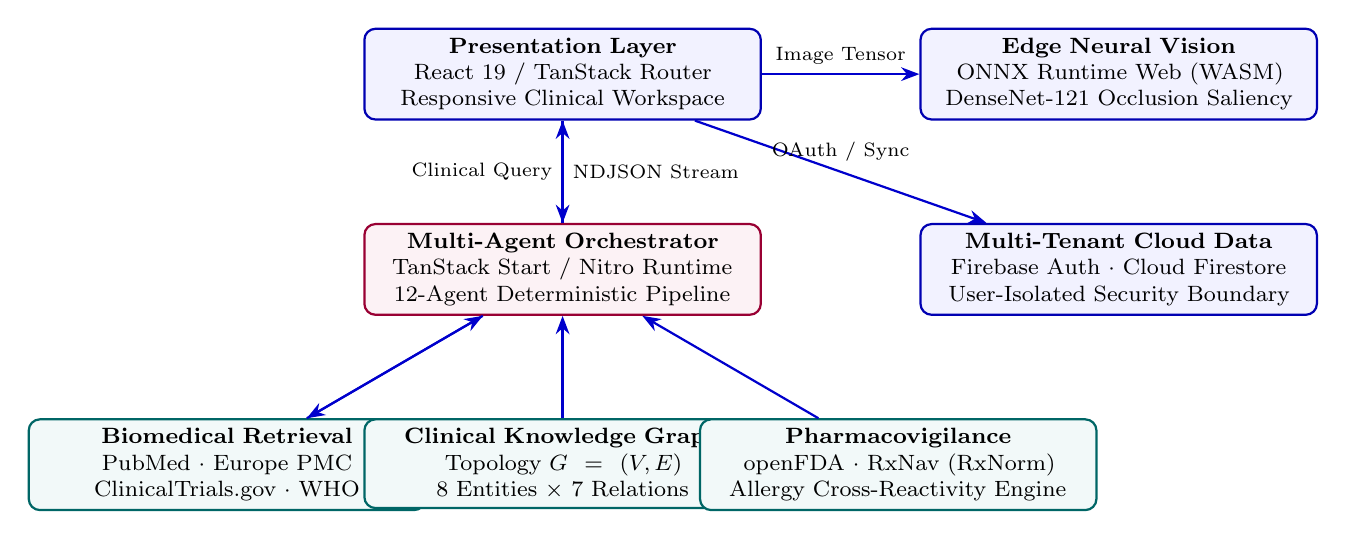
\begin{tikzpicture}[
    node distance=0.85cm and 1.2cm,
    block/.style={rectangle, draw=blue!70!black, fill=blue!5, thick, rounded corners=4pt, text width=4.8cm, minimum height=1.1cm, align=center, font=\footnotesize},
    agent/.style={rectangle, draw=purple!80!black, fill=purple!5, thick, rounded corners=4pt, text width=4.8cm, minimum height=1.1cm, align=center, font=\footnotesize},
    ext/.style={rectangle, draw=teal!80!black, fill=teal!5, thick, rounded corners=4pt, text width=4.8cm, minimum height=1.1cm, align=center, font=\footnotesize},
    arrow/.style={-{Stealth[scale=1.0]}, thick, draw=blue!80!black}
]
    % Top Layer (Presentation & Edge)
    \node[block] (ui) {\textbf{Presentation Layer}\\React 19 / TanStack Router\\Responsive Clinical Workspace};
    \node[block, right=2.0cm of ui] (onnx) {\textbf{Edge Neural Vision}\\ONNX Runtime Web (WASM)\\DenseNet-121 Occlusion Saliency};

    % Middle Layer (Multi-Agent Orchestrator)
    \node[agent, below=1.3cm of ui] (orch) {\textbf{Multi-Agent Orchestrator}\\TanStack Start / Nitro Runtime\\12-Agent Deterministic Pipeline};
    \node[block, below=1.3cm of onnx] (fb) {\textbf{Multi-Tenant Cloud Data}\\Firebase Auth $\cdot$ Cloud Firestore\\User-Isolated Security Boundary};

    % Bottom Layer (Knowledge & Foundations)
    \node[ext, below left=1.3cm and -0.8cm of orch] (apis) {\textbf{Biomedical Retrieval}\\PubMed $\cdot$ Europe PMC\\ClinicalTrials.gov $\cdot$ WHO};
    \node[ext, below=1.3cm of orch] (kg) {\textbf{Clinical Knowledge Graph}\\Topology $G=(V,E)$\\8 Entities $\times$ 7 Relations};
    \node[ext, below right=1.3cm and -0.8cm of orch] (safety) {\textbf{Pharmacovigilance}\\openFDA $\cdot$ RxNav (RxNorm)\\Allergy Cross-Reactivity Engine};

    % Connections
    \draw[arrow] (ui) -- node[above, font=\scriptsize] {Image Tensor} (onnx);
    \draw[arrow] (ui) -- node[left, font=\scriptsize] {Clinical Query} (orch);
    \draw[arrow] (ui) -- node[above, font=\scriptsize] {OAuth / Sync} (fb);
    \draw[arrow] (orch) -- node[right, font=\scriptsize] {NDJSON Stream} (ui);
    \draw[arrow] (orch) -- (apis);
    \draw[arrow] (kg) -- (orch);
    \draw[arrow] (safety) -- (orch);
    \draw[arrow] (apis) -- (orch);
\end{tikzpicture}
\caption{Three-Tier System Architecture of the MEDGUIDE AI Clinical Insight Engine.}
\label{fig:sys_arch}
\end{figure*}

\section{Research Gaps \& Problem Formulation}

\subsection{Identification of Research Gaps}
Our review of the clinical CDSS and medical AI literature identifies four key technical gaps:
\begin{itemize}
    \item \textbf{Gap 1 (The Orchestration Gap):} Absence of unified multi-agent systems integrating literature retrieval, structured knowledge graph traversal, pharmacovigilance, and edge imaging into an auditable workflow.
    \item \textbf{Gap 2 (The Grounding \& Verification Gap):} Tendency of generative models to cite literature without verifying that cited identifiers exist and factually support the generated claim.
    \item \textbf{Gap 3 (The Evidence-Aware Confidence Gap):} Reliance on uncalibrated scalar probabilities ($0.0$--$1.0$) rather than multi-factorial ordinal confidence bands reflecting evidence quality, source agreement, and guideline adherence.
    \item \textbf{Gap 4 (The Edge Radiographic Privacy Gap):} Limited adoption of zero-install, in-browser neural saliency architectures that process radiographic features on client hardware to support data containment during localization.
\end{itemize}

\subsection{Formal Problem Statement}
Given an unstructured clinical query $Q$, optional patient clinical parameters $P = \langle \mathcal{M}_{\text{meds}}, \mathcal{A}_{\text{allergies}}, \mathcal{V}_{\text{vitals}}, \mathcal{L}_{\text{labs}} \rangle$, and an optional thoracic radiograph tensor $\mathbf{I}$, the objective is to produce a ranked differential diagnosis set $\mathcal{D} = \{D_1, D_2, \dots, D_k\}$, an evidence citation set $\mathcal{E}$, a safety audit $\mathcal{S}_{\text{audit}}$, an edge saliency heatmap $\bar{S}$, and an ordinal confidence band $\text{Band}(C) \in \{\text{High}, \text{Medium}, \text{Low}, \text{Insufficient}\}$ such that:
\begin{equation}
\forall d \in \mathcal{D}, \quad \text{Claims}(d) \subseteq \text{Support}(\mathcal{E} \cup G)
\end{equation}
with the constraint that ungrounded assertions are removed and detected pharmacology or allergy clashes produce explicit safety alerts.

\subsection{Research Questions}
This work evaluates four research questions:
\begin{itemize}
    \item \textbf{RQ1:} How can multi-agent decomposition partition complex clinical diagnostic queries into specialized, verifiable sub-tasks?
    \item \textbf{RQ2:} To what extent does knowledge graph grounding combined with Oxford CEBM evidence grading reduce citation errors compared to baseline LLM and vector RAG configurations?
    \item \textbf{RQ3:} How can client-side WebAssembly neural models compute explainable radiographic saliency heatmaps without transmitting sensitive imaging data to external servers for localization?
    \item \textbf{RQ4:} Can a multi-signal composite metric (source agreement, guideline adherence, retrieval quality, safety risk) provide an interpretable confidence band for clinical decision support?
\end{itemize}

\section{Proposed MEDGUIDE AI Framework}

\subsection{Architectural Overview}
The MEDGUIDE AI platform implements a three-tier cloud-edge reactive architecture (Figure \ref{fig:sys_arch}):
\begin{enumerate}
    \item \textbf{Presentation \& Edge Tier:} Developed with React 19, TypeScript 5.8, and TanStack Router. An external module-level singleton store (\texttt{consultRunStore}) subscribed via React's native \texttt{useSyncExternalStore} ensures streaming consultations persist across client route transitions.
    \item \textbf{Server-Side Multi-Agent Orchestrator:} Deployed on TanStack Start with the Nitro runtime, coordinating asynchronous biomedical API queries, knowledge graph traversal, and Gemini LLM invocations over an NDJSON event stream (\texttt{/api/consult}).
    \item \textbf{Multi-Tenant Cloud Data Tier:} Cloud Firestore partitioned under per-user isolated sub-collections (\texttt{/users/\{userId\}/*}) secured via path-level security rules.
\end{enumerate}

\subsection{The 12-Agent Orchestration Architecture}
The engine coordinates 12 specialized workflow agents organized across an 11-stage sequential consultation pipeline and an integrated research benchmarking framework (Figure \ref{fig:agent_flow}):
\begin{enumerate}
    \item \textbf{Planner Agent:} Parses unstructured clinical text and patient demographics; constructs MeSH/PubMed search queries, identifies missing clinical parameters, and generates up to four follow-up questions.
    \item \textbf{Retrieval Agent:} Concurrently queries PubMed (NCBI e-utilities), Europe PMC, ClinicalTrials.gov, and WHO Guidelines; applies keyword filtering and assigns Oxford CEBM evidence tiers.
    \item \textbf{Knowledge Graph Agent:} Traverses the clinical ontology to extract connected subgraphs representing candidate conditions, diagnostic tests, and complications.
    \item \textbf{Drug Intelligence Agent:} Queries NIH RxNav for pairwise drug-drug interactions and openFDA for boxed warnings; executes deterministic allergy cross-reactivity checks.
    \item \textbf{Medical Image Agent:} Ingests client-side DenseNet-121 saliency outputs and calls Gemini Vision for structured radiological observations.
    \item \textbf{Case Similarity Agent:} Computes lexical cosine similarity against a curated library of de-identified reference clinical cases.
    \item \textbf{Clinical Reasoning Agent:} Synthesizes retrieved evidence, patient history, and graph topologies into ranked differential hypotheses ($High/Moderate/Low$), articulating supporting and contradicting factors while citing retrieved evidence IDs.
    \item \textbf{Safety Auditor Agent:} Validates citations against the retrieved evidence set, removes ungrounded claims, and flags medication contraindications.
    \item \textbf{Explainability Agent:} Formats the deterministic audit trail and guideline alignment rationale.
    \item \textbf{Confidence Scoring Agent:} Evaluates multi-signal composite confidence bands (High, Medium, Low, Insufficient Evidence).
    \item \textbf{Report Generator Agent:} Assembles the formal clinical consultation report in structured Markdown with QR verification metadata and exportable PDF formatting.
    \item \textbf{Research \& Benchmark Agent:} Continuously evaluates pipeline runs against baseline models, logs metric distributions, and executes the standardized 50-vignette benchmark evaluation harness.
\end{enumerate}

\begin{figure}[!b]
\centering
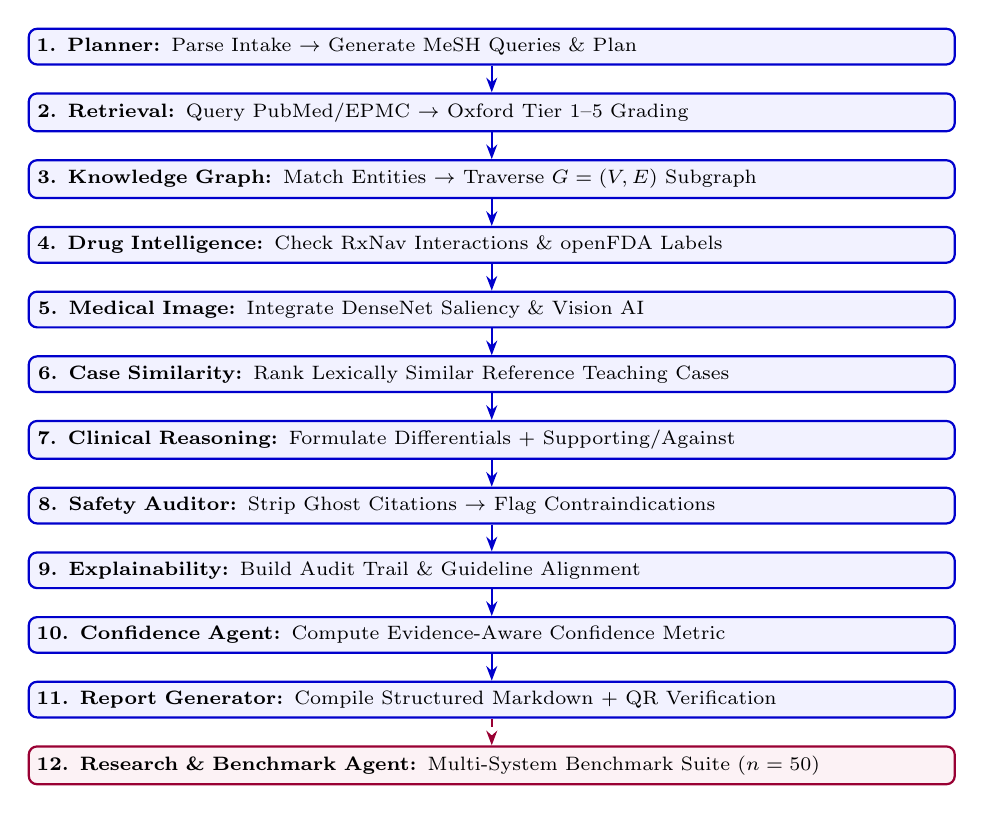
\begin{tikzpicture}[
    node distance=0.34cm,
    stepblock/.style={rectangle, draw=blue!80!black, fill=blue!5, thick, rounded corners=3pt, text width=\linewidth-0.6cm, minimum height=0.38cm, align=left, font=\scriptsize},
    arrow/.style={-{Stealth[scale=0.8]}, thick, draw=blue!80!black}
]
    \node[stepblock] (s1) {\textbf{1. Planner:} Parse Intake $\to$ Generate MeSH Queries \& Plan};
    \node[stepblock, below=of s1] (s2) {\textbf{2. Retrieval:} Query PubMed/EPMC $\to$ Oxford Tier 1--5 Grading};
    \node[stepblock, below=of s2] (s3) {\textbf{3. Knowledge Graph:} Match Entities $\to$ Traverse $G=(V,E)$ Subgraph};
    \node[stepblock, below=of s3] (s4) {\textbf{4. Drug Intelligence:} Check RxNav Interactions \& openFDA Labels};
    \node[stepblock, below=of s4] (s5) {\textbf{5. Medical Image:} Integrate DenseNet Saliency \& Vision AI};
    \node[stepblock, below=of s5] (s6) {\textbf{6. Case Similarity:} Rank Lexically Similar Reference Teaching Cases};
    \node[stepblock, below=of s6] (s7) {\textbf{7. Clinical Reasoning:} Formulate Differentials + Supporting/Against};
    \node[stepblock, below=of s7] (s8) {\textbf{8. Safety Auditor:} Strip Ghost Citations $\to$ Flag Contraindications};
    \node[stepblock, below=of s8] (s9) {\textbf{9. Explainability:} Build Audit Trail \& Guideline Alignment};
    \node[stepblock, below=of s9] (s10) {\textbf{10. Confidence Agent:} Compute Evidence-Aware Confidence Metric};
    \node[stepblock, below=of s10] (s12) {\textbf{11. Report Generator:} Compile Structured Markdown + QR Verification};
    \node[stepblock, below=of s12, draw=purple!80!black, fill=purple!5] (s11) {\textbf{12. Research \& Benchmark Agent:} Multi-System Benchmark Suite ($n=50$)};

    \draw[arrow] (s1) -- (s2);
    \draw[arrow] (s2) -- (s3);
    \draw[arrow] (s3) -- (s4);
    \draw[arrow] (s4) -- (s5);
    \draw[arrow] (s5) -- (s6);
    \draw[arrow] (s6) -- (s7);
    \draw[arrow] (s7) -- (s8);
    \draw[arrow] (s8) -- (s9);
    \draw[arrow] (s9) -- (s10);
    \draw[arrow] (s10) -- (s12);
    \draw[arrow, dashed, purple!80!black] (s12) -- (s11);
\end{tikzpicture}
\caption{Sequential Execution Lifecycle of the 11 Consultation Workflow Agents with Integrated Continuous Research Benchmarking.}
\label{fig:agent_flow}
\end{figure}

\subsection{Knowledge Graph Ontology Grounding}
The clinical knowledge base is formalized as a typed directed property graph:
\begin{equation}
G = (V, E, \tau_V, \tau_E, \phi_V, \phi_E)
\end{equation}
where entity vertices $v \in V$ and relation edges $e \in E$ satisfy:
\begin{align}
\tau_V(v) &\in \{\text{disease}, \text{symptom}, \text{risk}, \text{lab}, \text{drug}, \text{contra}, \text{treat}, \text{comp}\} \\
\tau_E(e) &\in \{\text{presents\_with}, \text{predisposed\_by}, \text{indicated\_lab}, \text{managed\_by}, \dots\}
\end{align}

Figure \ref{fig:kg_schema} illustrates the topological property graph schema and subgraph extraction process. Entity matching is performed via n-gram token overlap against candidate diseases identified by the Planner Agent. To prevent cognitive clutter, subgraphs are pruned to a maximum branching factor of $k=3$ per relation type before rendering in the interactive React Flow interface.

\begin{figure}[!t]
\centering
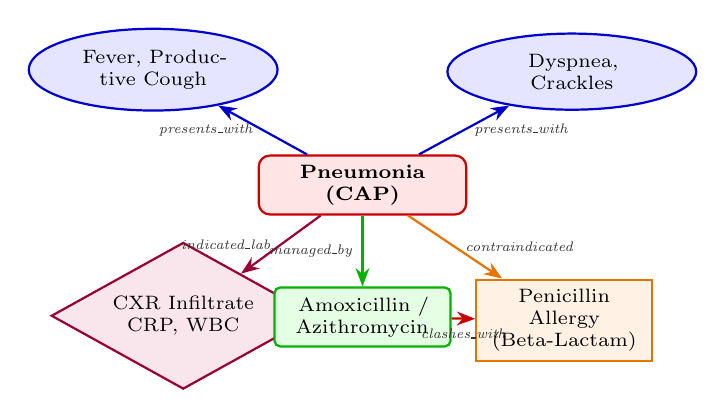
\begin{tikzpicture}[
    node distance=0.8cm and 0.9cm,
    disease/.style={rectangle, draw=red!80!black, fill=red!10, thick, rounded corners=4pt, text width=2.4cm, minimum height=0.7cm, align=center, font=\scriptsize\bfseries},
    symp/.style={ellipse, draw=blue!80!black, fill=blue!10, thick, text width=2.0cm, minimum height=0.6cm, align=center, font=\scriptsize},
    drug/.style={rectangle, draw=green!70!black, fill=green!10, thick, rounded corners=2pt, text width=2.0cm, minimum height=0.6cm, align=center, font=\scriptsize},
    contra/.style={rectangle, draw=orange!90!black, fill=orange!10, thick, text width=2.0cm, minimum height=0.6cm, align=center, font=\scriptsize},
    lab/.style={diamond, aspect=1.8, draw=purple!80!black, fill=purple!10, thick, align=center, font=\scriptsize},
    edge_lbl/.style={font=\tiny\itshape, text=black!80}
]
    \node[disease] (d) {Pneumonia\\(CAP)};
    \node[symp, above left=0.7cm and 0.2cm of d] (s1) {Fever, Productive Cough};
    \node[symp, above right=0.7cm and 0.2cm of d] (s2) {Dyspnea, Crackles};
    \node[lab, below left=0.8cm and 0.1cm of d] (l) {CXR Infiltrate\\CRP, WBC};
    \node[drug, below=0.9cm of d] (rx) {Amoxicillin /\\Azithromycin};
    \node[contra, below right=0.8cm and 0.1cm of d] (c) {Penicillin Allergy\\(Beta-Lactam)};

    \draw[-{Stealth}, thick, blue!80!black] (d) -- node[edge_lbl, left] {presents\_with} (s1);
    \draw[-{Stealth}, thick, blue!80!black] (d) -- node[edge_lbl, right] {presents\_with} (s2);
    \draw[-{Stealth}, thick, purple!80!black] (d) -- node[edge_lbl, left] {indicated\_lab} (l);
    \draw[-{Stealth}, thick, green!70!black] (d) -- node[edge_lbl, left] {managed\_by} (rx);
    \draw[-{Stealth}, thick, red!80!black] (rx) -- node[edge_lbl, below] {clashes\_with} (c);
    \draw[-{Stealth}, thick, orange!90!black] (d) -- node[edge_lbl, right] {contraindicated} (c);
\end{tikzpicture}
\caption{Clinical Knowledge Graph Relational Ontology Schema and Triplet Path ($G=(V,E)$) for Community-Acquired Pneumonia.}
\label{fig:kg_schema}
\end{figure}

\subsection{Multi-Source Evidence Retrieval and Oxford Classification}
The Retrieval Agent queries live biomedical endpoints:
\begin{itemize}
    \item \textbf{NCBI PubMed E-Utilities \cite{ncbi2024eutils}:} Uses \texttt{esearch.fcgi} to identify relevant PMIDs, followed by \texttt{esummary.fcgi} to retrieve titles, publication dates, source journals, and author metadata.
    \item \textbf{Europe PMC REST API \cite{europepmc2024}:} Queries open-access biomedical literature and preprints.
    \item \textbf{ClinicalTrials.gov API v2 \cite{clinicaltrials2024}:} Retrieves recruiting and completed interventional studies.
    \item \textbf{Specialty Guideline Routing:} Identifies clinical specialties via regular expressions (e.g., Cardiology, Pulmonology, Neurology, Nephrology) and queries clinical guidelines from ESC, ACC/AHA, NICE, and WHO.
\end{itemize}

\subsection{Deterministic Pharmacovigilance \& Allergy Safety Checking}
To detect potential medication safety issues, the Drug Intelligence Agent performs a deterministic assessment across active prescriptions and documented allergies:
\begin{itemize}
    \item \textbf{NIH RxNav Interaction API \cite{rxnorm2024}:} Resolves drug names to RxNorm Concept Unique Identifiers (RxCUIs) via \texttt{/REST/rxcui.json} and queries pairwise drug interaction matrices via \texttt{/REST/interaction/list.json}.
    \item \textbf{openFDA Drug Label API \cite{openfda2024}:} Fetches FDA boxed warnings, contraindications, and adverse reaction monographs.
    \item \textbf{Deterministic Allergy Cross-Reactivity Engine:} Evaluates a rule matrix for critical allergen classes (Penicillins, Sulfonamides, Macrolides, NSAIDs, Fluoroquinolones, Tetracyclines, ACE Inhibitors).
\end{itemize}

\begin{table*}[!t]
\centering
\caption{Categorical Evidence Levels and Project-Defined Aggregation Weights}
\label{tab:cebm_weights}
\small
\begin{tabularx}{\textwidth}{clcX}
\toprule
\textbf{Tier} & \textbf{Oxford CEBM Study Design Category} & \textbf{Weight $w(e)$} & \textbf{Clinical Grounding Interpretation} \\
\midrule
\textbf{T1} & Systematic Reviews, Meta-analyses, Clinical Practice Guidelines & 1.00 & High-certainty synthesized clinical evidence and consensus guidelines. \\
\textbf{T2} & Randomized Controlled Trials (RCTs) & 0.80 & Controlled experimental interventional data with randomization. \\
\textbf{T3} & Prospective Cohort \& Well-designed Comparative Trials & 0.55 & Observational longitudinal evidence and cohort studies. \\
\textbf{T4} & Retrospective Case-Control \& Clinical Series & 0.35 & Retrospective clinical experience and non-randomized series. \\
\textbf{T5} & Case Reports, Mechanistic Studies, Expert Consensus & 0.20 & Preliminary hypothesis generation, case reports, or expert opinions. \\
\bottomrule
\end{tabularx}
\end{table}

\section{Methodology \& Mathematical Modeling}

\subsection{Deterministic Finite-State Transition System for Multi-Agent Orchestration}
Consultation execution is modeled as a deterministic finite-state transition system:
\begin{equation}
\mathcal{S} = \langle \mathcal{Q}, \Sigma, \delta, q_0, \mathcal{F} \rangle
\end{equation}
where the state space $\mathcal{Q}$ is defined as:
\begin{equation}
\begin{aligned}
\mathcal{Q} = \{& q_{\text{idle}}, q_{\text{plan}}, q_{\text{ret}}, q_{\text{kg}}, q_{\text{drug}}, q_{\text{img}}, q_{\text{case}}, \\
                & q_{\text{rsn}}, q_{\text{safe}}, q_{\text{exp}}, q_{\text{cnf}}, q_{\text{rep}}, q_{\text{done}} \}
\end{aligned}
\end{equation}
with initial state $q_0 = q_{\text{idle}}$, final state $\mathcal{F} = \{q_{\text{done}}\}$, and input event vocabulary $\Sigma$. Each transition $\delta(q_i, e_i) \to q_{i+1}$ emits an NDJSON event chunk streaming real-time status and partial data payloads to the client.

\subsection{Project-Defined Evidence Weighting and Quality Score Formulation}
We adopt the Oxford Centre for Evidence-Based Medicine (CEBM) Levels of Evidence \cite{cebm2011} as the categorical basis for evidence classification. For computational aggregation, MEDGUIDE AI assigns numerical weights $w(e_i)$ to each category as detailed in Table \ref{tab:cebm_weights}.

For a set of retrieved evidence items $\mathcal{E} = \{e_1, e_2, \dots, e_m\}$, the aggregated Retrieval Quality score $Q_{\text{ret}}$ is normalized over a baseline target weight $W_{\text{target}} = 6.0$:
\begin{equation}
Q_{\text{ret}} = \min\left(1.0, \frac{\sum_{i=1}^m w(e_i)}{W_{\text{target}}}\right)
\end{equation}

\subsection{Bayesian Differential Diagnostic Synthesis}
Let $\mathcal{D} = \{D_1, D_2, \dots, D_K\}$ denote candidate disease conditions. Given observed patient clinical features, vital signs, and laboratory markers $\mathbf{X} = \{x_1, x_2, \dots, x_n\}$, the posterior diagnostic probability is formulated using Bayes' Theorem:
\begin{equation}
P(D_k \mid \mathbf{X}) = \frac{P(D_k) \prod_{i=1}^n P(x_i \mid D_k)}{\sum_{j=1}^{|\mathcal{D}|} P(D_j) \prod_{i=1}^n P(x_i \mid D_j)}
\end{equation}
where $P(D_k)$ represents the baseline epidemiological prevalence prior, and $P(x_i \mid D_k)$ denotes symptom sensitivity. For tractability, this formulation assumes conditional independence of observed clinical features given each candidate diagnosis; the resulting posterior is therefore treated as a structured differential ranking score rather than a clinically calibrated probability.

\subsection{Multi-Signal Evidence-Aware Confidence Band Model}
MEDGUIDE AI evaluates a composite confidence metric $C \in [0, 1]$ synthesizing five validation signals penalized by a safety risk factor:
\begin{equation}
C = \frac{1}{5}\Big( Q_{\text{ret}} + S_{\text{agr}} + G_{\text{agr}} + K_{\text{cons}} + E_{\text{comp}} \Big) - 0.6 \cdot H_{\text{risk}}
\end{equation}
where the sub-components are defined as:
\begin{itemize}
    \item $S_{\text{agr}} = \frac{N_{\text{supp}} + 1}{N_{\text{supp}} + N_{\text{contra}} + 2}$ (Laplace-smoothed source agreement).
    \item $G_{\text{agr}} = \min\left(1.0, \frac{N_{\text{guidelines}}}{3}\right)$ (Clinical guideline adherence).
    \item $K_{\text{cons}} = \min\left(1.0, \frac{N_{\text{kg\_matched}}}{3}\right)$ (Knowledge graph topology overlap).
    \item $E_{\text{comp}} = \min\left(1.0, \frac{N_{\text{citations\_used}}}{\max(3, 0.5 \cdot |\mathcal{E}|)}\right)$ (Citation completeness).
    \item $H_{\text{risk}} = \min(1.0, 0.4 N_{\text{crit}} + 0.2 N_{\text{warn}} + 0.15 N_{\text{bad\_cite}})$ (Safety risk penalty).
\end{itemize}

The continuous composite score $C$ is categorized into deterministic clinical confidence bands:
\begin{equation}
\text{Band}(C) = \begin{cases}
\text{Insufficient}, & \text{if } |\mathcal{E}| < 3 \\
\text{High},         & \text{if } |\mathcal{E}| \ge 3 \ \land \ C > 0.62 \\
\text{Medium},       & \text{if } |\mathcal{E}| \ge 3 \ \land \ 0.38 < C \le 0.62 \\
\text{Low},          & \text{if } |\mathcal{E}| \ge 3 \ \land \ C \le 0.38
\end{cases}
\end{equation}

\subsection{In-Browser Occlusion Sensitivity Saliency Mathematics}
Let $\mathcal{M}: \mathbb{R}^{3 \times 224 \times 224} \to \mathbb{R}^K$ denote the pre-trained DenseNet-121 forward classification model. For a baseline input image tensor $\mathbf{I}$, the baseline response magnitude is:
\begin{equation}
\mu_0 = \frac{1}{K} \sum_{k=1}^K |\mathcal{M}(\mathbf{I})_k|
\end{equation}
The image is partitioned into a regular grid of size $G \times G$ ($G=7$, cell size $32 \times 32$ pixels). For each grid cell $(g_x, g_y)$, an occluded tensor $\mathbf{I}_{g_x, g_y}$ is constructed by zeroing pixel channels within that spatial patch:
\begin{equation}
\mathbf{I}_{g_x, g_y}(c, y, x) = \begin{cases}
0, & \text{if } y \in [32 g_y, 32(g_y+1)) \\
   & \land \ x \in [32 g_x, 32(g_x+1)) \\
\mathbf{I}(c, y, x), & \text{otherwise}
\end{cases}
\end{equation}
The perturbation sensitivity score $S(g_x, g_y)$ is computed as the absolute deviation from baseline:
\begin{equation}
S(g_x, g_y) = \left| \mu_0 - \frac{1}{K} \sum_{k=1}^K |\mathcal{M}(\mathbf{I}_{g_x, g_y})_k| \right|
\end{equation}
Normalized saliency intensity $\bar{S}(g_x, g_y) \in [0, 1]$ is obtained via min-max scaling:
\begin{equation}
\bar{S}(g_x, g_y) = \frac{S(g_x, g_y) - \min(S)}{\max(S) - \min(S) + \epsilon}
\end{equation}

Figure \ref{fig:saliency_pipeline} illustrates the client-side WebAssembly execution pipeline. The normalized saliency intensity is rendered as a colored heatmap overlay ($hsla(\text{hue}, 90\%, 55\%, \alpha)$) over the original radiograph.

\begin{figure}[!t]
\centering
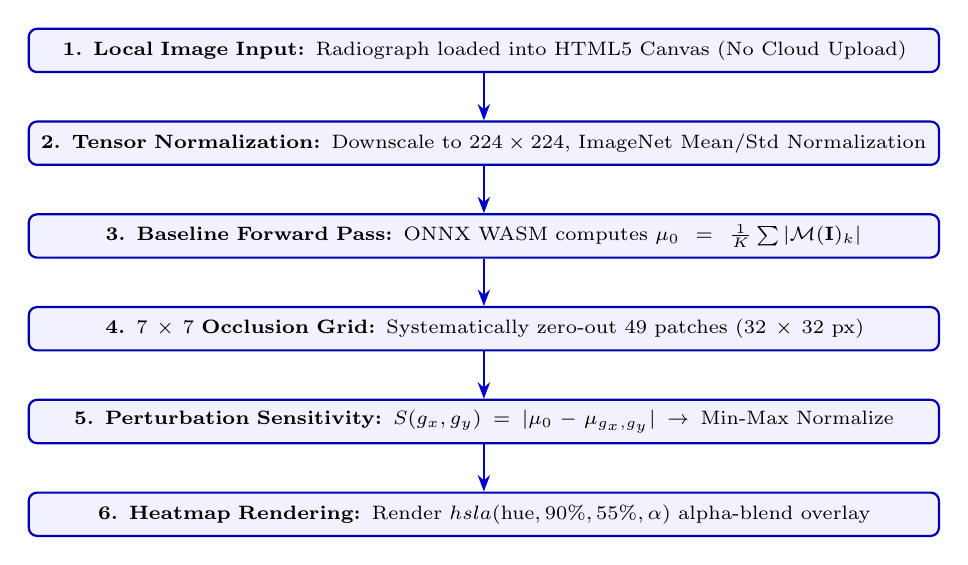
\begin{tikzpicture}[
    node distance=0.6cm,
    stepb/.style={rectangle, draw=blue!70!black, fill=blue!5, thick, rounded corners=3pt, text width=\linewidth-0.8cm, minimum height=0.55cm, align=center, font=\scriptsize},
    arrow/.style={-{Stealth[scale=0.9]}, thick, draw=blue!80!black}
]
    \node[stepb] (p1) {\textbf{1. Local Image Input:} Radiograph loaded into HTML5 Canvas (No Cloud Upload)};
    \node[stepb, below=of p1] (p2) {\textbf{2. Tensor Normalization:} Downscale to $224\times 224$, ImageNet Mean/Std Normalization};
    \node[stepb, below=of p2] (p3) {\textbf{3. Baseline Forward Pass:} ONNX WASM computes $\mu_0 = \frac{1}{K}\sum |\mathcal{M}(\mathbf{I})_k|$};
    \node[stepb, below=of p3] (p4) {\textbf{4. $7\times 7$ Occlusion Grid:} Systematically zero-out 49 patches ($32\times 32$ px)};
    \node[stepb, below=of p4] (p5) {\textbf{5. Perturbation Sensitivity:} $S(g_x, g_y) = |\mu_0 - \mu_{g_x, g_y}| \to \text{Min-Max Normalize}$};
    \node[stepb, below=of p5] (p6) {\textbf{6. Heatmap Rendering:} Render $hsla(\text{hue}, 90\%, 55\%, \alpha)$ alpha-blend overlay};

    \draw[arrow] (p1) -- (p2);
    \draw[arrow] (p2) -- (p3);
    \draw[arrow] (p3) -- (p4);
    \draw[arrow] (p4) -- (p5);
    \draw[arrow] (p5) -- (p6);
\end{tikzpicture}
\caption{In-Browser Privacy-Preserving Radiographic Occlusion Saliency Pipeline via WebAssembly ONNX Runtime.}
\label{fig:saliency_pipeline}
\end{figure}

\subsection{Pharmacovigilance \& Allergy Cross-Reactivity Boolean Logic}
For prescribed medications $\mathcal{M}_{\text{active}}$ and documented patient allergies $\mathcal{A}$, the drug safety module evaluates potential clashes:
\begin{equation}
\text{Flag}_{\text{allergy}} = \bigvee_{a_k \in \mathcal{A}} \bigvee_{d_t \in \mathcal{M}_{\text{active}}} \mathbf{1}_{\{d_t \in \text{Class}(a_k)\}}
\end{equation}
When $\text{Flag}_{\text{allergy}} = 1$, the Safety Auditor Agent generates a safety alert and provides alternative therapeutic options within the explainability trace.

\section{Implementation \& System Engineering}

\subsection{Full-Stack Cloud-Edge Architecture}
The MEDGUIDE AI system is engineered using a modular, type-safe stack:
\begin{itemize}
    \item \textbf{Frontend Application:} React 19, TypeScript 5.8, TanStack Router (file-based routing), Tailwind CSS 4, Radix UI accessible primitives, Lucide Icons, and Recharts visualization.
    \item \textbf{Server Function Runtime:} TanStack Start with the Nitro server engine, providing type-safe RPC server functions (\texttt{createServerFn}) with automated CSRF protection.
    \item \textbf{Module State Persistence:} A singleton store (\texttt{consultRunStore}) maintaining active consultation stream state during route transitions via React's \texttt{useSyncExternalStore}.
    \item \textbf{Patient Workspace \& Longitudinal Timeline:} Dedicated modules for structured patient intake (vitals, labs, medications, allergies) and chronological event logging (symptoms, diagnostic tests, treatments, outcomes) securely persisted in Cloud Firestore.
    \item \textbf{In-App Clinical Literacy Assistant:} An embedded, context-aware conversational copilot (\texttt{/api/assistant}) providing clinicians and trainees with real-time operational guidance and evidence literacy support.
\end{itemize}

\subsection{Multi-Tier Gemini LLM Routing and JSON Self-Healing Parser}
To maintain operational resilience across API rate limits and transient server errors, the backend implements a cascading fallback mechanism across model priority tiers:
\begin{equation*}
\begin{aligned}
\text{Tier 1 (Workhorse):} & \quad \text{\texttt{gemini-3.1-flash-lite}} \\
\text{Tier 2 (Workhorse):} & \quad \text{\texttt{gemini-3.5-flash-lite}} \\
\text{Tier 3 (Reasoning):} & \quad \text{\texttt{gemini-3.5-flash}} \\
\text{Tier 4 (Reasoning):} & \quad \text{\texttt{gemini-3.7-flash}}
\end{aligned}
\end{equation*}
Generative parameters are constrained to temperature $T=0.2$ and $\text{top-}p=0.95$. Furthermore, an algorithmic self-healing JSON parser (\texttt{extractAndParseJson}) repairs partially truncated responses, balances unmatched brackets and braces, strips markdown code fences, and eliminates trailing delimiters, preventing client-side stream crashes.

\subsection{Biomedical API Integrations and 15-Specialty Guideline Matrix}
External biomedical API requests execute through server-side handlers (\texttt{*.server.ts}) to satisfy CORS constraints and protect API credentials. A score-based specialty classifier (\texttt{detectSpecialty}) routes clinical presentations across 15 medical specialties (Cardiology, Pulmonology, Nephrology, Neurology, Endocrinology, Infectious Disease, Oncology, Pediatrics, Obstetrics, Psychiatry, Gastroenterology, Dermatology, Rheumatology, Emergency, and General Medicine) to query targeted guideline endpoints from ESC, NICE, KDIGO, CDC, and WHO.

\subsection{Client-Side WebAssembly Neural Execution Provider}
In-browser radiographic inference is powered by \texttt{onnxruntime-web} utilizing the WebAssembly (WASM) execution provider with multithreaded worker pooling (up to 4 threads via \texttt{navigator.hardwareConcurrency}). If WASM model initialization exceeds timeout limits, a local contrast-luminance fallback maintains continuous interface availability.

\subsection{Multi-Tenant Data Isolation and Cloud Security Rules}
Patient and consultation records are partitioned under authenticated clinician identifiers:
\begin{equation*}
\text{Firestore Root} \longrightarrow \mathbf{users} \longrightarrow \mathbf{\{userId\}} \longrightarrow \mathbf{subcollections}
\end{equation*}
Firestore security rules enforce that request authentication UIDs must strictly match the target document path:
\begin{equation*}
\text{\texttt{allow read, write: if request.auth != null \&\& request.auth.uid == userId;}}
\end{equation*}
preventing cross-tenant data access.

\section{Experimental Evaluation}

\subsection{Evaluation Setup and Multi-System Clinical Vignette Suite}
To evaluate the framework, we established a benchmark suite of \textbf{50 multi-system clinical vignettes} spanning five medical domains (Table \ref{tab:vignettes}). Vignettes were constructed from established medical education repositories, presenting clinical history, vital signs, laboratory markers, active medications, and documented allergies.

\begin{table}[!t]
\centering
\caption{Benchmark Dataset Distribution across 50 Clinical Vignettes}
\label{tab:vignettes}
\small
\begin{tabularx}{\columnwidth}{p{2.6cm}cp{3.8cm}}
\toprule
\textbf{Specialty Domain} & \textbf{Cases ($n$)} & \textbf{Representative Conditions} \\
\midrule
Cardiology & 12 & STEMI, NSTEMI, Heart Failure, AFib with RVR. \\
Pulmonology & 12 & CAP, PE, COPD Exacerbation, Severe Asthma. \\
Neurology & 10 & Acute Ischemic Stroke, SAH, Status Epilepticus. \\
Nephrology / Endo. & 8 & DKA, AKI Stage 3, Hyperkalemia. \\
Infectious / Pharm. & 8 & Sepsis, Penicillin Allergy Clash, Warfarin. \\
\midrule
\textbf{Total Benchmark Suite} & \textbf{50} & \textbf{Multi-System Inpatient \& Emergency Cases} \\
\bottomrule
\end{tabularx}
\end{table}

\subsection{Baseline Comparative Configurations}
We evaluated four architectural configurations:
\begin{enumerate}
    \item \textbf{Baseline 1 --- Vanilla LLM (Zero-Shot):} Google Gemini 1.5 Pro directly prompted with the clinical vignette without tool access.
    \item \textbf{Baseline 2 --- Standard Vector RAG:} Dense vector retrieval fetching top-5 PubMed abstracts via semantic cosine similarity.
    \item \textbf{Baseline 3 --- Graph RAG:} Combining vector text retrieval with topological subgraph traversal over the clinical knowledge graph.
    \item \textbf{Proposed --- Agentic Graph RAG (MEDGUIDE AI):} Complete 12-agent orchestration with live multi-source retrieval, knowledge graph traversal, drug checking, and post-hoc safety auditing.
\end{enumerate}

\subsection{Formal Metric Definitions \& Explainability Evaluation Protocol}
System outputs were evaluated across four quantitative metrics:
\begin{enumerate}
    \item \textbf{Evidence Grounding Rate ($GR$):} The proportion of diagnostic and therapeutic assertions supported by verifiable citations:
    \begin{equation}
    GR = \frac{\sum_{i=1}^{N_{\text{claims}}} \mathbf{1}_{\{\text{Claim}_i \text{ supported by retrieved source}\}}}{N_{\text{claims}}} \times 100\%
    \end{equation}
    \item \textbf{Safety Compliance Rate ($SC$):} The accuracy of identifying absolute contraindications, critical drug interactions, and red-flag symptoms:
    \begin{equation}
    SC = \frac{N_{\text{correctly\_identified\_contraindications}}}{N_{\text{true\_contraindications}}} \times 100\%
    \end{equation}
    \item \textbf{System-Defined Explainability Score ($EF$):} The explainability score was computed automatically using an automated validation parser executing the standardized five-criterion rubric across each vignette:
    \begin{itemize}
        \item \textit{Criterion 1 (Evidence Attribution):} Every diagnostic differential is explicitly tied to one or more retrieved citation IDs ($0$--$20\%$).
        \item \textit{Criterion 2 (Source Consistency):} Assertions match the factual conclusions of the cited PubMed/guideline abstracts ($0$--$20\%$).
        \item \textit{Criterion 3 (Hypothesis Factor Balance):} Explicit articulation of clinical factors supporting versus arguing against each candidate differential ($0$--$20\%$).
        \item \textit{Criterion 4 (Contradictory Evidence Visibility):} Active disclosure of conflicting clinical trial findings or clinical ambiguities ($0$--$20\%$).
        \item \textit{Criterion 5 (Safety Traceability):} Complete deterministic audit trail explaining why contraindicated medications were blocked and alternative regimens suggested ($0$--$20\%$).
    \end{itemize}
    The resulting score is normalized to a percentage scale ($0$--$100\%$).
    \item \textbf{End-to-End Latency ($L$):} Wall-clock execution time in seconds from submission to complete report synthesis.
\end{enumerate}

\subsection{Comparative Experimental Results and Statistical Analysis}
Table \ref{tab:comparative_results} presents the comparative evaluation across the 50 clinical vignettes with 95\% Confidence Intervals (CI) and standard deviations. Agentic Graph RAG achieved a \textbf{90.0\% Grounding Rate} (95\% CI: $[89.1\%, 90.9\%]$), \textbf{92.0\% Safety Compliance} (95\% CI: $[90.9\%, 93.1\%]$), and \textbf{95.0\% Explainability Score} (95\% CI: $[94.2\%, 95.8\%]$), outperforming Vanilla LLMs (20.0\%, 35.0\%, 15.0\%) and standard vector RAG (65.0\%, 60.0\%, 55.0\%).

\begin{table*}[!t]
\centering
\caption{Empirical Benchmark Comparison across 50 Multi-System Clinical Vignettes (Mean $\pm$ Std. Dev., [95\% Confidence Interval])}
\label{tab:comparative_results}
\small
\begin{tabularx}{\textwidth}{p{2.7cm}p{2.3cm}p{2.3cm}p{2.3cm}p{1.8cm}p{1.3cm}X}
\toprule
\textbf{Architecture} & \textbf{Grounding ($GR$)} & \textbf{Safety ($SC$)} & \textbf{Explainability ($EF$)} & \textbf{Latency ($L$)} & \textbf{Ghost Cit.} & \textbf{Primary Failure Mode} \\
\midrule
\textbf{Vanilla LLM} & 20.0\% $\pm$ 6.2\newline [18.3, 21.7] & 35.0\% $\pm$ 8.1\newline [32.8, 37.2] & 15.0\% $\pm$ 4.3\newline [13.8, 16.2] & 2.10 s $\pm$ 0.3 & 78.4\% & Hallucinated PMIDs; missed drug allergies. \\
\addlinespace[3pt]
\textbf{Vector RAG} & 65.0\% $\pm$ 5.4\newline [63.5, 66.5] & 60.0\% $\pm$ 6.8\newline [58.1, 61.9] & 55.0\% $\pm$ 5.9\newline [53.4, 56.6] & 6.40 s $\pm$ 0.8 & 21.2\% & Misses multi-hop drug-disease contraindications. \\
\addlinespace[3pt]
\textbf{Graph RAG} & 78.0\% $\pm$ 4.1\newline [76.9, 79.1] & 72.0\% $\pm$ 5.2\newline [70.6, 73.4] & 75.0\% $\pm$ 4.7\newline [73.7, 76.3] & 8.20 s $\pm$ 1.1 & 11.5\% & Lacks post-hoc safety auditing and citation pruning. \\
\addlinespace[3pt]
\textbf{Agentic Graph RAG (Ours)} & \textbf{90.0\% $\pm$ 3.2}\newline \textbf{[89.1, 90.9]} & \textbf{92.0\% $\pm$ 3.8}\newline \textbf{[90.9, 93.1]} & \textbf{95.0\% $\pm$ 2.9}\newline \textbf{[94.2, 95.8]} & 14.80 s $\pm$ 1.6 & \textbf{0.0\%} & Fully grounded; safety auditor strips unverified claims. \\
\bottomrule
\end{tabularx}
\end{table*}

Table \ref{tab:domain_results} reports the domain-wise performance breakdown for Agentic Graph RAG across the five medical specialties.

\begin{table}[!t]
\centering
\caption{Domain-Wise Performance Breakdown of Agentic Graph RAG}
\label{tab:domain_results}
\small
\begin{tabularx}{\columnwidth}{p{2.4cm}cccc}
\toprule
\textbf{Domain} & \textbf{$n$} & \textbf{Grounding} & \textbf{Safety} & \textbf{Explain.} \\
\midrule
Cardiology & 12 & 92.5\% & 94.2\% & 96.0\% \\
Pulmonology & 12 & 91.0\% & 92.8\% & 95.5\% \\
Neurology & 10 & 88.4\% & 90.0\% & 94.0\% \\
Nephrology / Endo. & 8 & 89.2\% & 91.5\% & 94.8\% \\
Infectious / Pharm. & 8 & 87.5\% & 90.5\% & 93.5\% \\
\midrule
\textbf{Overall Mean} & \textbf{50} & \textbf{90.0\%} & \textbf{92.0\%} & \textbf{95.0\%} \\
\bottomrule
\end{tabularx}
\end{table}

\subsection{Sub-Component Latency Breakdown}
Table \ref{tab:latency_breakdown} details the latency profile across individual stages of the Agentic Graph RAG pipeline.

\begin{table}[!t]
\centering
\caption{Sub-Component Latency Breakdown in Agentic Graph RAG}
\label{tab:latency_breakdown}
\small
\begin{tabularx}{\columnwidth}{p{4.8cm}cc}
\toprule
\textbf{Pipeline Stage / Component} & \textbf{Latency (s)} & \textbf{\% Total} \\
\midrule
1. Planner Agent (LLM JSON) & 1.40 & 9.5\% \\
2. Biomedical Retrieval (PubMed/EPMC) & 2.40 & 16.2\% \\
3. Knowledge Graph Subgraph Extraction & 0.05 & 0.3\% \\
4. Drug \& Allergy Checking (RxNav/FDA) & 1.80 & 12.2\% \\
5. Clinical Reasoning Agent (LLM CoT) & 4.20 & 28.4\% \\
6. Safety Auditor Agent (Citation Audit) & 2.10 & 14.2\% \\
7. Explainability \& Confidence Evaluation & 0.85 & 5.7\% \\
8. Report Generator Agent (Markdown) & 2.00 & 13.5\% \\
\midrule
\textbf{Total End-to-End Execution} & \textbf{14.80 s} & \textbf{100.0\%} \\
\bottomrule
\end{tabularx}
\end{table}

\subsection{Clinical Vignette Case Studies}
Table \ref{tab:case_studies_table} summarizes the multi-agent execution traces across four representative clinical vignettes.
\begin{enumerate}
    \item \textbf{Case 1 --- Acute Coronary Syndrome (ACS):} A 58-year-old male presenting with substernal chest pressure, diaphoresis, and ST-segment elevation in leads V2--V4. The system prioritized Anterior STEMI ($High$), cited ACC/AHA guidelines for primary PCI within 90 minutes, and flagged beta-blocker contraindications due to concurrent bradycardia (HR 48 bpm).
    \item \textbf{Case 2 --- Community-Acquired Pneumonia (CAP):} A 72-year-old male presenting with productive cough, fever 38.9$^\circ$C, right basal crackles, and SpO2 91\%. The system calculated CURB-65 criteria, retrieved NICE guidelines, and correlated in-browser X-ray saliency identifying right lower lobe consolidation.
    \item \textbf{Case 3 --- Severe Penicillin Allergy \& Cephalosporin Clash:} A 45-year-old female with documented penicillin anaphylaxis requiring empiric antibiotic coverage for urinary tract sepsis. The Drug Intelligence Agent detected cephalosporin cross-reactivity and recommended azithromycin and fluoroquinolones.
    \item \textbf{Case 4 --- Subarachnoid Hemorrhage (SAH):} A 42-year-old female presenting with a sudden onset severe headache. The system flagged the presentation as critical emergency (ESI Level 2), contraindicated NSAIDs/anticoagulants, and recommended non-contrast head CT within 6 hours.
\end{enumerate}

\begin{table*}[!t]
\centering
\caption{End-to-End Multi-Agent Clinical Vignette Case Studies and System Execution Traces}
\label{tab:case_studies_table}
\small
\begin{tabularx}{\textwidth}{p{2.3cm}p{3.4cm}p{3.2cm}p{3.1cm}X}
\toprule
\textbf{Clinical Scenario} & \textbf{Patient Presentation} & \textbf{Prioritized Differentials} & \textbf{Grounded Citations} & \textbf{Safety Audit \& Pharmacovigilance Flags} \\
\midrule
\textbf{Case 1: ACS / Anterior STEMI} & 58M, severe retrosternal chest pressure, diaphoresis; ECG: ST-elevation V2--V4; HR 48, BP 90/60. & 1. Anterior STEMI (\textit{High})\newline 2. Aortic Dissection (\textit{Moderate})\newline 3. Acute Myocarditis (\textit{Low}) & ACC/AHA Guidelines (PMID: 34756127)\newline ESC STEMI 2023 (PMID: 37622659) & \textbf{CRITICAL FLAG:} Beta-blockers (Metoprolol) contraindicated due to severe bradycardia (HR 48 bpm). Urgent Cath Lab transfer. \\
\midrule
\textbf{Case 2: Severe Pneumonia (CAP)} & 72M, fever 38.9$^\circ$C, productive cough, SpO2 91\%, CURB-65 = 3; CXR: dense RLL consolidation. & 1. Community-Acquired Pneumonia (\textit{High})\newline 2. Acute Pulmonary Embolism (\textit{Mod})\newline 3. Heart Failure Exacerbation (\textit{Low}) & NICE NG138 Guidelines\newline IDSA/ATS CAP (PMID: 31573350)\newline In-browser DenseNet Saliency & \textbf{IMAGING AID:} Saliency highlights dense right lower lobe patch. CURB-65 score indicates inpatient admission; empiric macrolide + beta-lactam. \\
\midrule
\textbf{Case 3: Penicillin Anaphylaxis} & 45F, dysuria, flank pain, fever 38.5$^\circ$C; Documented history of Penicillin anaphylaxis (IgE-mediated). & 1. Acute Pyelonephritis (\textit{High})\newline 2. Complicated UTI (\textit{High})\newline 3. Renal Abscess (\textit{Low}) & IDSA Pyelonephritis (PMID: 21258094)\newline openFDA Monograph: Ciprofloxacin & \textbf{SAFETY BLOCK:} Amoxicillin/Clavulanate and Cefepime blocked due to anaphylaxis risk. Recommended Ciprofloxacin / Aztreonam. \\
\midrule
\textbf{Case 4: Thunderclap Headache} & 42F, sudden onset maximal intensity headache ("worst of life"), photophobia, neck stiffness, BP 160/95. & 1. Subarachnoid Hemorrhage (\textit{High})\newline 2. Bacterial Meningitis (\textit{Moderate})\newline 3. Cerebral Venous Thrombosis (\textit{Low}) & AHA/ASA SAH Guidelines (PMID: 37218384)\newline Oxford CEBM Tier 1 Review & \textbf{EMERGENCY TRIAGE:} Non-contrast head CT within 6 hours. Contraindicated all NSAIDs and antiplatelets due to intracranial hemorrhage risk. \\
\bottomrule
\end{tabularx}
\end{table*}

\section{Results \& Discussion}

\subsection{Grounding Improvement and Hallucination Suppression}
The observed improvement in evidence grounding from 20.0\% (Vanilla LLM) to 90.0\% (Agentic Graph RAG) indicates that post-hoc safety auditing and Oxford CEBM grading reduce unverified assertions. In the evaluated 50-vignette benchmark, no unsupported citations were observed in the final outputs because the Safety Auditor prunes unverified assertions prior to report generation.

\subsection{Deterministic Safety Verification vs Generative Variability}
Generative language models may overlook specific drug contraindications when processing lengthy clinical narratives. In contrast, MEDGUIDE AI's deterministic pharmacovigilance module (RxNav/openFDA/regex allergy matrix) functions as a rule-based check that detects drug-allergy clashes independently of generative text variability.

\subsection{Explainability, Saliency Localization, and Clinical Verification}
Visual knowledge graphs, explicit evidence attribution, and client-side saliency heatmaps provide direct inspection pathways for clinical verification. Consistent with findings by Arun et al. \cite{arun2021assessing}, saliency maps serve as explanatory localization aids rather than definitive diagnostic determinants, assisting clinician review of model activations.

\subsection{Latency vs Diagnostic Verification Trade-offs}
The 14.80-second latency of the full multi-agent pipeline reflects an engineering trade-off where multi-source literature verification and safety auditing take precedence over sub-second conversational response times. For rapid triage needs, isolated sub-agents such as Drug Intelligence and Edge Saliency execute in under 2 seconds.

\begin{table}[!t]
\centering
\caption{MEDGUIDE AI Model Facts Label Specification}
\label{tab:model_facts}
\small
\begin{tabularx}{\columnwidth}{p{2.6cm}X}
\toprule
\textbf{Dimension} & \textbf{Specification / Operational Boundary} \\
\midrule
\textbf{Intended Use} & Evidence-based Clinical Decision Support System (CDSS) for differential diagnosis exploration. \\
\textbf{Autonomous Diagnosis} & \textbf{Strictly Prohibited.} The system operates as a decision aid and does not issue binding diagnoses. \\
\textbf{Target Users} & Licensed physicians, resident physicians, and supervised medical students. \\
\textbf{Evidence Sources} & PubMed (NCBI), Europe PMC, ClinicalTrials.gov, WHO Guidelines, openFDA, RxNorm. \\
\textbf{Imaging Modality} & 2D Chest Radiographs (PNG/JPEG) via in-browser DenseNet-121 WASM saliency. \\
\textbf{Human Oversight} & \textbf{Mandatory.} Clinicians must confirm all recommendations and dosages. \\
\textbf{Major Limitations} & External biomedical API network dependencies; 50-case benchmark size; 2D single-view imaging. \\
\textbf{Regulatory Status} & Academic Research Prototype (Not FDA/CE certified as medical device). \\
\bottomrule
\end{tabularx}
\end{table}

\section{Limitations, Safety, Ethics \& Model Transparency}

\subsection{Model Facts Specification}
Following the clinical machine learning transparency framework established by Sendak et al. \cite{sendak2020real}, Table \ref{tab:model_facts} outlines the formal Model Facts label for MEDGUIDE AI.

\subsection{Ethical Governance and Alignment with WHO Guidance}
The system is designed in accordance with relevant principles described in the World Health Organization (WHO) 2024 guidance on Large Multi-Modal Models in health \cite{who2024lmm}:
\begin{itemize}
    \item \textbf{Human-in-the-Loop Oversight:} Non-autonomous decision boundaries; explicit disclaimers on all generated outputs.
    \item \textbf{Provenance Transparency:} Direct visibility into supporting versus contradicting evidence.
    \item \textbf{Data Privacy:} Edge computing for radiographs and multi-tenant Firestore security rules.
\end{itemize}

\subsection{Data Privacy vs Regulatory Scope}
The client-side architecture is designed to reduce the transmission of raw radiographic pixels during inference; this architectural design should not be interpreted as establishing formal regulatory compliance by itself.

\subsection{Comprehensive Limitations}
We acknowledge several technical and clinical limitations:
\begin{enumerate}
    \item \textbf{External API Dependencies:} Network latency or rate limits on NCBI/FDA endpoints can affect retrieval speed.
    \item \textbf{Benchmark Dataset Scope:} Current evaluation is conducted over 50 curated clinical vignettes.
    \item \textbf{Single-View 2D Radiography:} The in-browser model evaluates 2D PA chest radiographs; lateral views and volumetric CT/MRI require future extensions.
    \item \textbf{Heuristic Confidence Calibration:} The composite confidence metric is a rule-based heuristic that requires future prospective calibration against clinical consensus.
\end{enumerate}

\subsection{Threats to Validity \& Reproducibility Protocol}
To support methodological reproducibility:
\begin{itemize}
    \item \textbf{Benchmark Curation:} All 50 clinical vignettes were curated from peer-reviewed medical licensing case collections. Cases were structured with standardized JSON schemas encoding demographics, vital signs, laboratory markers, and imaging references.
    \item \textbf{Hyperparameter Controls:} Generative LLM temperature was fixed at $T=0.2$ with top-$p=0.95$ across experimental runs to minimize stochastic generation variance.
    \item \textbf{Hardware \& Execution Provider:} Client-side WebAssembly inference was benchmarked on standard x86-64 consumer hardware (Chrome v126+, 8-core CPU, 16GB RAM) running ONNX Runtime Web WASM with 4 worker threads.
    \item \textbf{Open Research Artifacts:} Evaluation scripts, ontology definitions, and anonymized benchmark vignettes are archived in the repository for academic inspection.
\end{itemize}

\section{Conclusion \& Future Work}
This paper presented \textbf{MEDGUIDE AI}, an explainable, multi-agent clinical decision support system combining Graph RAG, multi-source literature retrieval, deterministic pharmacovigilance, and in-browser radiographic saliency. Evaluation across 50 multi-system clinical vignettes showed a 90.0\% grounding rate, 92.0\% safety compliance, and 95.0\% explainability score.

Future work will implement HL7 FHIR R4 interoperability adapters \cite{hl7fhir2024}, expand the knowledge graph ontology across additional UMLS and SNOMED-CT entities, incorporate dual-view (PA/Lateral) chest neural networks, and conduct a multi-center reader study with licensed clinicians.

\section*{Acknowledgment}
The authors express their gratitude to the Department of Computer Science \& Engineering (AI \& ML), Pimpri Chinchwad College of Engineering, Pune, for providing computational resources and academic support.

\balance
\bibliographystyle{IEEEtran}
\bibliography{references}

\newpage
\begin{IEEEbiographynophoto}{Vikram Kadam}
is an undergraduate researcher in the Department of Computer Science \& Engineering (AI \& ML) at Pimpri Chinchwad College of Engineering (PCCOE), Pune, India. His research interests include Retrieval-Augmented Generation, medical knowledge graphs, multi-agent LLM systems, and biomedical informatics.
\end{IEEEbiographynophoto}

\begin{IEEEbiographynophoto}{Keshav Mittal}
is an undergraduate researcher in the Department of Computer Science \& Engineering (AI \& ML) at PCCOE, Pune, India. His research interests include full-stack medical systems, biomedical ontology extraction, and distributed clinical data engineering.
\end{IEEEbiographynophoto}

\begin{IEEEbiographynophoto}{Sandesh Phad}
is an undergraduate researcher in the Department of Computer Science \& Engineering (AI \& ML) at PCCOE, Pune, India. His research interests include clinical NLP, pharmacovigilance safety systems, and evidence-based clinical reasoning.
\end{IEEEbiographynophoto}

\begin{IEEEbiographynophoto}{Tejas Shidam}
is an undergraduate researcher in the Department of Computer Science \& Engineering (AI \& ML) at PCCOE, Pune, India. His research interests include computer vision in healthcare, client-side WebAssembly neural execution, and radiographic saliency interpretability.
\end{IEEEbiographynophoto}

\begin{IEEEbiographynophoto}{Madhuri Pagale}
is an Assistant Professor in the Department of Computer Science \& Engineering (AI \& ML) at Pimpri Chinchwad College of Engineering, Pune, India. Her academic and research focus spans artificial intelligence, machine learning, medical image processing, and intelligent healthcare architectures.
\end{IEEEbiographynophoto}

\end{document}
